\chapter{MetaTrader 5专家顾问开发经验}
\label{chap:mt5}

\section{概述}

本章记录了在MetaTrader 5中开发专家顾问(EA)的经验,总结适用于Alpha挖掘系统的经验教训。MT5平台提供了完整的交易基础设施,可以为Mini-WorldQuant系统的设计提供参考。

\section{MT5架构}

\subsection{专家顾问结构}

MT5 EA遵循结构化生命周期:

\begin{figure}[h]
\centering
\begin{tikzpicture}[
    node distance=1.2cm,
    init/.style={ellipse, draw=green!50, fill=green!10, thick, minimum width=2cm, minimum height=0.8cm, text centered},
    process/.style={rectangle, draw=blue!50, fill=blue!10, thick, minimum width=2.5cm, minimum height=0.8cm, text centered, rounded corners},
    decision/.style={diamond, draw=red!50, fill=red!10, thick, minimum width=1.5cm, minimum height=1cm, text centered, aspect=2},
    action/.style={rectangle, draw=orange!50, fill=orange!10, thick, minimum width=2cm, minimum height=0.8cm, text centered, rounded corners},
    arrow/.style={->, >=stealth, thick}
]
    % Lifecycle
    \node[init] (start) {OnInit()};
    \node[process, below=of start] (init) {Initialize\\Indicators};
    \node[process, below=of init] (setup) {Setup Trade\\Object};
    
    % Main loop
    \node[process, below=of setup, yshift=-0.3cm] (tick) {OnTick()};
    \node[decision, below=of tick, yshift=-0.3cm] (check) {Trading\\Allowed?};
    \node[process, below=of check, yshift=-0.3cm] (update) {Update\\Indicators};
    \node[decision, below=of update, yshift=-0.3cm] (position) {Position\\Open?};
    
    % Position management
    \node[action, below=of position, yshift=-0.3cm, xshift=-2cm] (manage) {Manage\\Position};
    \node[action, below=of position, yshift=-0.3cm, xshift=2cm] (signal) {Check\\Signals};
    
    % Actions
    \node[action, below=of manage] (close) {Close\\Position};
    \node[action, below=of signal] (open) {Open\\Position};
    
    % Cleanup
    \node[init, below=of close, xshift=2cm] (deinit) {OnDeinit()};
    
    % Arrows
    \draw[arrow] (start) -> (init);
    \draw[arrow] (init) -> (setup);
    \draw[arrow] (setup) -> (tick);
    \draw[arrow] (tick) -> (check);
    \draw[arrow] (check) -> node[right] {Yes} (update);
    \draw[arrow] (check) -| node[above] {No} ++(-2,0) |- (tick);
    \draw[arrow] (update) -> (position);
    \draw[arrow] (position) -> node[left] {Yes} (manage);
    \draw[arrow] (position) -> node[right] {No} (signal);
    \draw[arrow] (manage) -> (close);
    \draw[arrow] (signal) -> (open);
    \draw[arrow] (close) -> (deinit);
    \draw[arrow] (open) -> (deinit);
    \draw[arrow, dashed, bend left=60] (deinit) to (tick);
    
    % Loop label
    \node[right=0.5cm of tick, font=\small] {Main Loop};
\end{tikzpicture}
\caption{MT5专家顾问生命周期}
\label{fig:mt5-lifecycle}
\end{figure}

\begin{lstlisting}[style=mql5, caption=基本EA结构]
//+------------------------------------------------------------------+
//| Expert initialization function                                   |
//+------------------------------------------------------------------+
int OnInit()
{
   // Initialize indicators
   rsi_handle = iRSI(_Symbol, TimeFrame, RSI_Period, RSI_Applied_Price);
   if(rsi_handle == INVALID_HANDLE)
   {
      return(INIT_FAILED);
   }
   
   // Initialize trade object
   trade.SetExpertMagicNumber(MagicNumber);
   trade.SetDeviationInPoints(Slippage);
   trade.SetTypeFilling(ORDER_FILLING_FOK);
   
   return(INIT_SUCCEEDED);
}

//+------------------------------------------------------------------+
//| Expert tick function                                             |
//+------------------------------------------------------------------+
void OnTick()
{
   // Check if we have enough bars
   if(Bars(_Symbol, TimeFrame) < RSI_Period + 2)
   {
      return;
   }
   
   // Update indicator values
   if(!UpdateRSI())
   {
      return;
   }
   
   // Check for existing position
   CheckExistingPosition();
   
   // Check for new entry signals
   if(!position_open)
   {
      CheckEntrySignals();
   }
}

//+------------------------------------------------------------------+
//| Expert deinitialization function                                 |
//+------------------------------------------------------------------+
void OnDeinit(const int reason)
{
   if(rsi_handle != INVALID_HANDLE)
      IndicatorRelease(rsi_handle);
}
\end{lstlisting}

\subsection{关键组件}

\subsubsection{交易管理}

\begin{lstlisting}[style=mql5, caption=交易执行]
void OpenBuyPosition()
{
   double ask = SymbolInfoDouble(_Symbol, SYMBOL_ASK);
   
   if(trade.Buy(LotSize, _Symbol, ask, 0, 0, "RSI Scalping Buy"))
   {
      position_ticket = trade.ResultOrder();
      position_open = true;
      current_position_type = POSITION_TYPE_BUY;
   }
}

void ClosePosition()
{
   if(PositionSelectByTicket(position_ticket))
   {
      trade.PositionClose(position_ticket);
      position_open = false;
      position_ticket = 0;
      rsi_against_position = false;
      bars_against_count = 0;
   }
}
\end{lstlisting}

\subsubsection{信号检测}

\begin{lstlisting}[style=mql5, caption=入场信号逻辑]
void CheckEntrySignals()
{
   // Buy signal: RSI crosses from oversold to above oversold
   if(rsi_two_bars_ago <= RSI_Oversold && rsi_prev > RSI_Oversold)
   {
      OpenBuyPosition();
   }
   
   // Sell signal: RSI crosses from overbought to below overbought
   if(rsi_two_bars_ago >= RSI_Overbought && rsi_prev < RSI_Overbought)
   {
      OpenSellPosition();
   }
}
\end{lstlisting}

\begin{figure}[h]
\centering
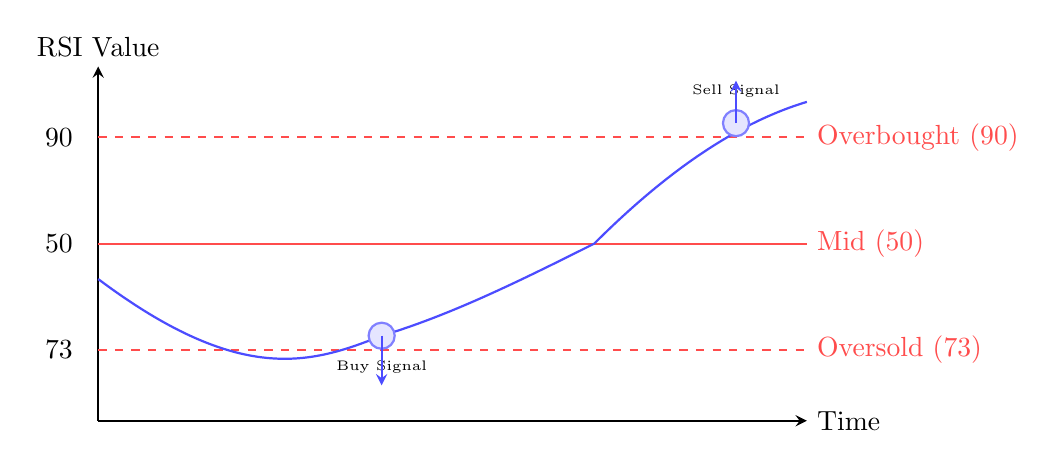
\begin{tikzpicture}[
    scale=0.9,
    axis/.style={->, >=stealth, thick},
    signal/.style={circle, draw=blue!50, fill=blue!10, thick, minimum size=0.3cm},
    level/.style={thick, color=red!70},
    arrow/.style={->, >=stealth, thick, blue!70}
]
    % RSI axis
    \draw[axis] (0,0) -- (0,5) node[above] {RSI Value};
    \draw[axis] (0,0) -- (10,0) node[right] {Time};
    
    % RSI levels
    \draw[level, dashed] (0,4) -- (10,4) node[right] {Overbought (90)};
    \draw[level, dashed] (0,1) -- (10,1) node[right] {Oversold (73)};
    \draw[level] (0,2.5) -- (10,2.5) node[right] {Mid (50)};
    
    % RSI curve
    \draw[thick, blue!70] (0,2) .. controls (2,0.5) and (3,0.8) .. (4,1.2)
                         .. controls (5,1.5) and (6,2) .. (7,2.5)
                         .. controls (8,3.5) and (9,4.2) .. (10,4.5);
    
    % Signal points
    \node[signal] at (4,1.2) {};
    \node[below=0.2cm] at (4,1.2) {\tiny Buy Signal};
    \draw[arrow] (4,1.2) -> (4,0.5);
    
    \node[signal] at (9,4.2) {};
    \node[above=0.2cm] at (9,4.2) {\tiny Sell Signal};
    \draw[arrow] (9,4.2) -> (9,4.8);
    
    % Labels
    \node[left=0.2cm] at (0,4) {90};
    \node[left=0.2cm] at (0,1) {73};
    \node[left=0.2cm] at (0,2.5) {50};
\end{tikzpicture}
\caption{RSI信号检测:交叉模式}
\label{fig:mt5-signals}
\end{figure}

\subsubsection{持仓管理}

\begin{lstlisting}[style=mql5, caption=持仓监控]
void CheckExistingPosition()
{
   if(!position_open)
   {
      return;
   }
   
   // Check if position still exists
   if(!PositionSelectByTicket(position_ticket))
   {
      position_open = false;
      position_ticket = 0;
      return;
   }
   
   // Exit conditions based on RSI target
   if(current_position_type == POSITION_TYPE_BUY)
   {
      // Check if RSI is against the position
      if(rsi_current < RSI_Oversold)
      {
         if(!rsi_against_position)
         {
            rsi_against_position = true;
            bars_against_count = 1;
         }
         else
         {
            bars_against_count++;
         }
         
         // Close position if RSI has been against for Y bars
         if(bars_against_count >= BarsToWait)
         {
            ClosePosition();
            return;
         }
      }
      else
      {
         // RSI is no longer against, reset counter
         if(rsi_against_position)
         {
            rsi_against_position = false;
            bars_against_count = 0;
         }
         
         // Exit long position when RSI reaches buy target
         if(rsi_current >= RSI_Target_Buy)
         {
            ClosePosition();
         }
      }
   }
}
\end{lstlisting}

\section{经验教训}

\subsection{健壮性模式}

\subsubsection{错误处理}

\begin{lstlisting}[style=mql5, caption=健壮的错误处理]
bool IsTradingAllowed()
{
   // Check if market is open
   if(!SymbolInfoInteger(_Symbol, SYMBOL_TRADE_MODE))
   {
      return false;
   }
   
   // Check if spread is acceptable
   double spread = SymbolInfoDouble(_Symbol, SYMBOL_ASK) - 
                   SymbolInfoDouble(_Symbol, SYMBOL_BID);
   int spreadInPips = (int)(spread / _Point);
   
   if(spreadInPips > MaxSpread)
   {
      return false;
   }
   
   // Check if enough bars available
   if(Bars(_Symbol, TimeFrame) < RSI_Period + 2)
   {
      return false;
   }
   
   return true;
}
\end{lstlisting}

\subsubsection{会话管理}

\begin{lstlisting}[style=mql5, caption=基于会话的交易]
bool IsAsianSession()
{
   MqlDateTime dt;
   TimeToStruct(TimeCurrent(), dt);
   
   int hour = dt.hour;
   
   // Asian session: 00:00 - 09:00 GMT
   if(hour >= 0 && hour < 9)
   {
      return true;
   }
   
   return false;
}

void OnTick()
{
   // Check if trading is allowed
   if(!IsTradingAllowed())
   {
      return;
   }
   
   // Check if we're in Asian session
   if(!IsAsianSession())
   {
      // Close all positions if outside session
      if(CloseOutsideSession && !sessionCloseAttempted)
      {
         CloseAllTrades("Outside Asian session");
         sessionCloseAttempted = true;
      }
      return;
   }
   else
   {
      sessionCloseAttempted = false;
   }
   
   // ... trading logic
}
\end{lstlisting}

\subsection{性能优化}

\subsubsection{高效的指标更新}

\begin{lstlisting}[style=mql5, caption=优化的指标访问]
bool UpdateRSI()
{
   if(CopyBuffer(rsi_handle, 0, 0, 3, rsi_buffer) < 3)
   {
      return false;
   }
   
   rsi_current = rsi_buffer[0];  // Current bar
   rsi_prev = rsi_buffer[1];     // Previous bar
   rsi_two_bars_ago = rsi_buffer[2];  // Two bars ago
   
   return true;
}
\end{lstlisting}

\subsubsection{基于K线的处理}

\begin{lstlisting}[style=mql5, caption=新K线检测]
void OnTick()
{
   // Check if this is a new bar
   datetime current_bar_time = iTime(_Symbol, TimeFrame, 0);
   if(current_bar_time == last_bar_time)
   {
      return;  // Still the same bar, don't process
   }
   
   last_bar_time = current_bar_time;
   
   // Process only on new bar
   // ... trading logic
}
\end{lstlisting}

\section{在Alpha挖掘中的应用}

\subsection{实时执行模式}

适用于Alpha执行的MT5模式:

\begin{enumerate}
    \item \textbf{事件驱动架构}:OnTick()模式用于实时处理
    \item \textbf{状态管理}:跟踪持仓状态和信号状态
    \item \textbf{风险管理}:点差检查、会话过滤器、持仓规模
    \item \textbf{错误恢复}:优雅处理API失败
\end{enumerate}

\subsection{Alpha到交易的流水线}

\begin{lstlisting}[language=Python, caption=Alpha执行系统]
class AlphaExecutor:
    """Execute alphas in real-time trading"""
    
    def __init__(self, broker_connection):
        self.broker = broker_connection
        self.active_positions = {}
        self.alpha_signals = {}
        
    def on_market_update(self, market_data: dict):
        """Called on each market tick (similar to OnTick)"""
        # Update all active alphas
        for alpha_id, alpha in self.active_alphas.items():
            # Evaluate alpha expression
            signal = self.evaluate_alpha(alpha, market_data)
            
            # Check for position changes
            if signal != self.alpha_signals.get(alpha_id):
                self.handle_signal_change(alpha_id, signal, market_data)
                self.alpha_signals[alpha_id] = signal
    
    def evaluate_alpha(self, alpha: AlphaResult, market_data: dict) -> float:
        """Evaluate alpha expression with current market data"""
        # Parse and evaluate alpha expression
        # Similar to MT5 indicator evaluation
        return self.expression_evaluator.evaluate(alpha.template, market_data)
    
    def handle_signal_change(self, alpha_id: str, signal: float, 
                            market_data: dict):
        """Handle signal change (similar to MT5 position management)"""
        current_position = self.active_positions.get(alpha_id)
        
        # Determine target position
        if signal > 0.5:
            target_position = 'LONG'
        elif signal < -0.5:
            target_position = 'SHORT'
        else:
            target_position = 'FLAT'
        
        # Adjust position if needed
        if current_position != target_position:
            if current_position:
                self.close_position(alpha_id)
            
            if target_position != 'FLAT':
                self.open_position(alpha_id, target_position, market_data)
\end{lstlisting}

\section{最佳实践}

\subsection{代码组织}

\begin{itemize}
    \item \textbf{模块化函数}:分离信号检测、持仓管理、风险管理
    \item \textbf{配置参数}:使用输入参数便于优化
    \item \textbf{魔术数字}:使用唯一的魔术数字进行持仓识别
    \item \textbf{错误日志}:全面的日志记录用于调试
\end{itemize}

\subsection{风险管理}

\begin{itemize}
    \item \textbf{持仓规模}:基于账户权益的动态手数大小
    \item \textbf{止损/止盈}:始终设置风险限制
    \item \textbf{最大点差}:当点差过大时过滤交易
    \item \textbf{会话过滤器}:仅在最优会话期间交易
\end{itemize}

\subsection{测试}

\begin{itemize}
    \item \textbf{策略测试器}:使用MT5策略测试器进行回测
    \item \textbf{可视化测试}:可视化模式用于调试
    \item \textbf{优化}:使用遗传算法优化参数
    \item \textbf{前瞻测试}:在实盘前在模拟账户上测试
\end{itemize}

\section{与Alpha挖掘的集成}

\subsection{Alpha到EA的转换}

\begin{lstlisting}[language=Python, caption=Alpha到MT5 EA转换器]
class AlphaToEAConverter:
    """Convert alpha expressions to MT5 Expert Advisors"""
    
    def convert_alpha_to_ea(self, alpha: AlphaResult) -> str:
        """Generate MQL5 code from alpha expression"""
        # Parse alpha expression
        expression_tree = self.parse_expression(alpha.template)
        
        # Generate EA code
        ea_code = f"""
//+------------------------------------------------------------------+
//| Generated EA from Alpha: {alpha.template[:50]}
//+------------------------------------------------------------------+
#property copyright "Auto-Generated"
#property version   "1.00"

#include <Trade\\Trade.mqh>

input double LotSize = 0.1;
input int MagicNumber = {hash(alpha.template) % 100000};
input int Slippage = 3;

CTrade trade;
{self.generate_indicator_handles(expression_tree)}
{self.generate_signal_logic(expression_tree)}
{self.generate_position_management(alpha)}

int OnInit() {{
   {self.generate_initialization(expression_tree)}
   return(INIT_SUCCEEDED);
}}

void OnTick() {{
   {self.generate_tick_logic(expression_tree, alpha)}
}}

void OnDeinit(const int reason) {{
   {self.generate_cleanup(expression_tree)}
}}
"""
        return ea_code
    
    def generate_signal_logic(self, tree) -> str:
        """Generate signal detection logic"""
        # Convert expression tree to MQL5 signal logic
        # Example: ts_rank(ts_delta(close, 1), 20) > 0.7
        return """
double signal = CalculateAlpha();
if(signal > 0.7 && !HasPosition()) {
   OpenBuyPosition();
} else if(signal < -0.7 && !HasPosition()) {
   OpenSellPosition();
}
"""
\end{lstlisting}

\section{总结}

MT5专家顾问开发为以下方面提供了有价值的模式:
\begin{itemize}
    \item 实时事件驱动架构
    \item 健壮的错误处理和状态管理
    \item 风险管理和持仓规模
    \item 性能优化技术
    \item 测试和验证方法
\end{itemize}

这些模式直接指导Mini-WorldQuant交易执行系统的设计,确保健壮、生产就绪的Alpha部署。
